\documentclass[10pt]{beamer}

\usetheme{moloch}

\usepackage{booktabs}
\usepackage[scale=2]{ccicons}

\usepackage{pgfplots}
\usepgfplotslibrary{dateplot}
\usepackage{tikzpeople}
\usepackage{tikz}
\usetikzlibrary{overlay-beamer-styles}
\usetikzlibrary{backgrounds}

\usepackage{fontawesome5}
\usepackage{amsmath}
\usepackage{amssymb}
\newcommand{\kkk}{\mathbf{k}}
\newcommand{\KKK}{\mathbf{K}}
\newcommand{\rrr}{\mathbf{r}}
\newcommand{\iNTT}{$\mathsf{iNTT}$}
\newcommand{\bch}{\mathsf{BCH}}
\newcommand{\intt}{\mathsf{iNTT}}
\newcommand{\leap}{\textsc{Leap}}
\usepackage{xcolor}
\definecolor{mBGcol}{HTML}{fafafa}
\definecolor{colA}{HTML}{990099}
\definecolor{colC}{HTML}{b6b6b6}
\definecolor{colB}{HTML}{00b300}
\definecolor{colD}{HTML}{2eb8b8}
\definecolor{thirdColor}{HTML}{6A5ACD}


\newcommand{\bv}[1]{\mathbf{#1}}
\usepackage[lambda,landau,operators,probability,sets,logic,advantage,complexity,asymptotics,notions,mm,primitives,ff,adversary,advantage]{cryptocode}


\title{Symmetric-Style Oblivious Lattice Evaluation}
\subtitle{Or: OPRFs for the symmetric cryptographer}
\date{26$^{th}$ of November, 2025}
\author{Lena Heimberger}
\institute{NTU Singapore, School of Physical and Mathematical Sciences}
\titlegraphic{\vspace{-2em}
\includegraphics[height=1cm]{figures/logo.pdf}\hfill
\includegraphics[height=1cm]{figures/NTU_Logo.png}}
\pgfplotsset{compat=1.18}

\begin{document}

\maketitle

\begin{frame}
  \frametitle{Hi!}
  \begin{itemize}
    \item PhD student @Graz University of Technology \\ Supervisor:
      Christian Rechberger\pause
    \item I study lattice-based OPRFs from heuristic assumptions to get
      \emph{efficient} OPRFs. \pause
    \item Recently built an OPRF more efficient than elliptic
      curves!~\cite{EC:HKLMRR25}\pause
    \item Needs more analysis- especially the underlying PRF\\ joint work with
      Sonja Denk (Master student @ TUG)

  \end{itemize}
\end{frame}

% Brief intro to OPRFs: what they are and why we care
% Key applications: private set intersection, password-authenticated key exchange, privacy-preserving authentication
% Real-world motivation: Why PSI matters for contact discovery, private databases, threat intelligence sharing

\begin{frame}
  \frametitle{Motivation for Oblivious Pseudorandom Functions}
  \begin{itemize}
    \item simple(r) primitive from asymmetric cryptography\pause
    \item gives rise to a number of cool constructions
    \item cheap! \pause...pre-quantum
  \end{itemize}
  \begin{exampleblock}{Pseudorandom Function}
    A pseudorandom function~(PRF) \cite{C:GolGolMic84,GolGolMic86} is a
    deterministic and polynomial time function $F \colon
    \{0,1\}^k\times\{0,1\}^x\rightarrow \{0,1\}^y$ such that
    there is no probabilistic polynomial-time algorithm
    to distinguish any output $y$ from a randomly chosen element from $\{0,1\}^y$.
    \label{def:prf}
  \end{exampleblock}
\end{frame}

\begin{frame}
  \frametitle{Definitions}
  \centering
  \begin{tikzpicture}[every node/.style={minimum width=1.5cm},scale=0.8]

    \node[alice, monitor, shirt=blue!40!black, minimum size=1.5cm, label=Client] (alice)
      {};
    \node[scale=2.67, label=Server, xshift=3.5cm] (server) {{\large{\faServer}}};
    \node[scale=2.67, label=compute, xshift=1.9cm] (hashfunction) {\({y
      \coloneqq F_k(c)}\)};

    \node(Alicetext) [below of=alice,xshift=1cm, yshift=-0.8cm,text
      width=3cm, text=gray]{input \(c \in \mathcal{C}\), gets \(y\)};;
    \node(Servertext) [below of=server, xshift=0.5cm,yshift=-0.5cm,text
      width=3cm,text=gray]{key \(k\in \mathcal{K}\)};;
  \end{tikzpicture}
  \begin{exampleblock}{Oblivious Pseudorandom Function}
    An oblivious pseudorandom function~(OPRF)~\cite{TCC:FIPR05} is a protocol between two parties. One
    party holds the secret key $k$ and the other holds their secret input $x$.
    The OPRF privately realizes the joint computation outputting $F_k(x)$ for a PRF $F$ to the
    party holding $x$, and nothing to the party holding $k$.
    \label{def:oprf}
  \end{exampleblock}

\end{frame}

\begin{frame}{Additional Properties}
  \begin{description}
    \item[Partial Obliviousness] In a POPRF, the client submits a tag $t$ in addition to the
      input $x$ and gets the evaluation $y
      \coloneqq F_k (t, x)$. $t$ contains  additional information,
      e.g. a validity period.\pause
    \item[Threshold] Get a valid evaluation from a $t$-out-of-$n$ servers.\pause
    \item[Verifiability] The client can ensure that a pre-commited server key $k$ was used to compute $y = F_k
      (x)$. \\ VOPRF+POPRF=VPOPRF\pause
    \item[Public Verifiability] means we built a blind signature.
  \end{description}
\end{frame}

\begin{frame}
  \frametitle{Motivation for (PQ)OPRFs @ CATF}
  \begin{tikzpicture}[overlay, remember picture]
    \node at ([xshift=-1cm, yshift=-0.5cm]current page.north east) { % Adjust xshift and yshift for padding
        
\includegraphics[width=2cm]{figures/catf.jpg}
      };
  \end{tikzpicture}
  \begin{itemize}
    \item Underlying primitives are not well-studied\pause
    \item Example: Crypto Dark Matter PRF~\cite{TCC:BIPSW18}\footnote{~$\odot$
      is component-wise multiplication}: \\ 
      \vspace{-1em}
      \begin{align*}
        F(k,x)\coloneqq \bv{B}\cdot_3 [\bv{A}\cdot_2 (k\odot_2 x)]
      \end{align*}

      low-depth wPRF  in a single round of computation \footnote{~after
      preprocessing}\pause
    \item existing attacks on dark matter (O)PRFs: \pause
      \begin{itemize}
        \item \cite{PKC:CCKK21} lower DM expectations, \cite{JohMeiNgu23}:
          even better attack\pause
        \item \cite{EPRINT:CheJan25} use secret information in ciphertexts to break verifiability of: 
          \begin{itemize}
            \item vADDG~\cite{EC:ADDG24}: proposed 80 bits of security; attack estimates 10
            \item Replication and Polynomial encoding
              schemes~\cite{CCS:CKPTH24}: $\mathbb{P}_{\text{successful
              forgery}}= 1$, linear
              time complexity\pause
          \end{itemize}
        \item \cite{EPRINT:SidWan25} bring the attack of~\cite{FSE:MadRad25}
          under the birthday bound and make it appicable to more parameters.
          This breaks $\frac{3}{4}$ of the constructions in \emph{Improved alternating-moduli PRFs}~\cite{C:APRR24}
      \end{itemize}
  \end{itemize}
\end{frame}

\begin{frame}
  \frametitle{Motivation for (PQ)OPRFs @ SPMS}
    \begin{tikzpicture}[overlay, remember picture]
      \node[fill=mBGcol] at ([xshift=-1.8cm, yshift=-0.5cm]current page.north east) { % Adjust xshift and yshift for padding
              \includegraphics[scale=0.26]{figures/SPMS_logo.png}
          };
      \end{tikzpicture}
  \begin{itemize}
    \item Post-Quantum Cryptography is a good excuse to do hard math\pause
    \item MSCS: Cool engineering challenges!\pause
    \item Math: Lower bounds are not clear\pause
    \item Example: Learning with Rounding~(LWR) PRFs
      \begin{itemize}
        \item \cite{EC:BanPeiRos12}: modulus has to be exponential in input
          length
        \item 
          Spring PRF~\cite{FSE:BBLPR14}: large modulus seems to be a proof
          artifact
      \end{itemize}
  \end{itemize}
  %  \footnote{~$\odot$
  %          is component-wise multiplication}: \\ 
  %  \onslide<3-6>{
  %  }

\end{frame}


\begin{frame}
  \frametitle{Table of Contents}
 %  \setbeamertemplate{section in toc}[sections numbered]
  \tableofcontents
\end{frame}

% \begin{frame}
%   \frametitle{Graz? }
% 
%   \begin{figure}
%     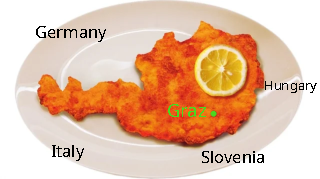
\includegraphics[scale=1.5]{figures/graz.pdf}
%     \caption{Schnitzel map from
%     \url{https://www.reddit.com/r/mapporncirclejerk/comments/e3x9h4/map\_of\_austria\_but\_its\_actually\_a\_schnitzel/},
%     modified by me. }
%   \end{figure}
% 
% \end{frame}
% 

\section{Lattices, so symmetric: SPRING }
\begin{frame}{Naor-Reingold PRF~\cite{NaoRei04}}
  \begin{itemize}
    \item The Naor-Reingold PRF~\cite{NaoRei04} that generically builds a PRF
      from an Abelian group action $*$.\pause
    \item
      To compute the PRF over $m$ input bits, we sample $m+1$ group elements $[g_0,
      g_1, \ldots, g_m]$. \pause
    \item Start with group action with $g_0$\pause
    \item For every following
      group element, the group action is performed when the $i^{th}$ bit of the input is set. \pause
  \end{itemize}
  \begin{example}[Naor-Reingold with seven input bits]
    For example, for $0110111$ we would
    compute the group action $g_0*g_2*g_3*g_5*g_6*g_7$.
  \end{example}
\end{frame}

\begin{frame}{Learning with Rounding PRFs}
  \begin{itemize}
    \item \emph{derandomize} Learning with errors \pause
      \begin{itemize}
        \item SIS: $\bv{As}=\bv{x}$
        \item LWE: add noise to get approximate solution $\bv{As}+\bv{e}=\bv{x}$
        \item LWR: round from big modulus $p$ to smaller modulus $q$\\ 
          $\lfloor\bv{As}_q\rceil_p$\pause
      \end{itemize}
    \item NIST PKE/KEM Finalist: Saber~\cite{NISTPQC-R3:SABER20}\pause
    \item Naor-Reingold PRF from LWR: 
  \end{itemize}
  \onslide<1->{
    \begin{align*}
      \mathcal{F}_{\bv{K}}(c_1,
      \cdots,c_m)=S\left(\bv{k}_0 \prod_{i=1}^m \bv{k}_{i}^{c_i}\right)
    \end{align*}
  }


\end{frame}

\begin{frame}{\textsc{Spring} is a lattice-based PRF}
  \begin{itemize}
    \item 2014: \alert{heuristic} LWR PRF with small modulus\pause
    \item two modes: \pause
      \begin{itemize}
        \item \textsc{Spring-BCH} with $q=257$\pause
        \item \textsc{Spring-CRT} with $q=514$\pause
      \end{itemize}
    \item \cite{EC:HKLMRR25} focus in \textsc{Spring-BCH}: rounding bias reduction using extended BCH code
      $[128,64,22]$\pause
  \end{itemize}

  \onslide<3-6>{
    \begin{figure}[H]
      \label{Spring:PRF}
      \vspace{-1em}
      \begin{align*}
        \mathcal{F}_{\bv{K}}(c_1,
        \cdots,c_m)=S\left(\kkk_0 \prod_{i=1}^m \kkk_{i}^{c_i}\right)
      \end{align*}
    \end{figure}
  }

  \onslide<7>{
    \begin{figure}[H]
      \label{Spring:PRF-intt}
      \vspace{-8em}
      \begin{align*}
        \mathcal{F}_{\bv{K}}(c_1,
        \cdots,c_m)=S\left(\intt\left(\kkk_0\odot \prod_{i=1}^m \kkk_{i}^{c_i}\right)\right)
      \end{align*}
    \end{figure}
  }

  \onslide<8>{
    \begin{figure}[H]
      \label{Spring:PRF-intt-lookup}
      \vspace{-8em}
      \begin{align*}
        \mathcal{F}_{\bv{K}}(c_1,
        \cdots,c_m)=S\left(\intt\left(\mathsf{lookup}\left(\kkk_0+
        \sum_{i=1}^m {c_i}\kkk_{i}\right)\right) \right)
      \end{align*}
    \end{figure}
    Multiplication is addition of exponents! \\ 
    \vspace*{-1em}
    \begin{align*}
      g^ag^b= g^{a+b}~\text{for some generator $g$}
    \end{align*}
  }
\end{frame}

\begin{frame}{Why $q=\{257\}$?}
  \begin{itemize}
    \item Choice of modulus from ease of implementation: 
    \item $q=257$
      \begin{itemize}
        \item only use \emph{invertable} polynomials \pause \\ 
        \item Computation mod $q$: use units (nonzero coefficients) \pause \\
          avoid zeroing out 
        \item Fermat's Theorem for prime $q$: 
          \begin{align*}
            g^{q-1}\equiv g^0 \equiv 1 \mod q 
          \end{align*}\pause
        \item use subset-sum of exponents instead of multiplication \pause
        \item Sample in exponent form $\mod q-1= 256$\pause \\ 
          fits in a single byte!
      \end{itemize}
  \end{itemize}
\end{frame}

\begin{frame}{Why $q=\{514\}$?}
  \begin{itemize}
    \item Even modulus $q=514=2*257$\pause
    \item 257-component as on previous slide\pause
    \item 2-component $R_2^*$; 257-style\pause\\ 
      polynomial multiplication $\rightarrow$ coefficient multiplication
      $\rightarrow$ coefficient addition
      \begin{itemize}
        \item polynomial is \emph{invertible} when sum of coefficients is
          odd\pause
        \item Polynomial is represented in \emph{power representation}:
          $A(x)=x^0+b_1x^1+b_2x^2+...+b_{127}x^{127}, b_i\in \{0,1\}$\pause \\
        \item We'll have to change the presentation twice before combination with 257-component \pause
        \item \alert{Spoiler} the end result will look a lot like a symmetric
          cipher!

      \end{itemize}
  \end{itemize}
\end{frame}
 \begin{frame}{OPRF-friendly $q$}
   \begin{itemize}
     \item some issues with $q=257$ and oblivious evaluation\pause \\
       \alert{maybe later}\pause
     \item PRF needs to be fast, OPRF, esp. from lattices, needs to have small
       communications\pause
     \item We need some distance between $p$ and $q$, $\approx 3$ bits\pause
     \item Compose out of $\mod 2$ constructions: $q=16=2*2*2*2$
   \end{itemize}
 \end{frame}

 \section{Almost a symmetric cipher:\\ Spring mod 16}

 \begin{frame}{Symmetric structure}
   \vspace*{-2em}
   \begin{figure}[H]
     \begin{align*}
       \mathcal{F}_{\bv{K}}(c_1, \cdots, c_m) = \uncover<4->{\color{colD}}S\left(
         \uncover<3->{\color{thirdColor}} \intt\left(
           \uncover<2->{\color{colA}} \mathsf{lookup}\left(
             \uncover<1->{\color{colB} \kkk_0 + \sum_{i=1}^m {c_i}\kkk_{i}}
           \right)
         \right)
       \right)
     \end{align*}
   \end{figure}\pause
   \begin{itemize}
     \item {\color{colB} Key addition }\pause
     \item {\color{colA}Substitution }\pause
     \item {\color{thirdColor}Permutation }\pause
     \item {\color{colD}Truncation}\pause
     \item Optional round function through CTR mode for longer outputs
   \end{itemize}
 \end{frame}

 \begin{frame}{Efficient Subset-Products}
   Let's zoom into the computation $\mod 2$
   \vspace*{-2em}
   \begin{figure}[H]
     \begin{align*}
       \mathcal{F}_{\bv{K}}(c_1, \cdots, c_m) = S\left(
         \intt\left(
           \mathsf{lookup}\left(
             \uncover<1->{{\color{colB} \kkk_0 + \sum_{i=1}^m {c_i}\kkk_{i}}}
           \right)
         \right)
       \right)
     \end{align*}
   \end{figure}
   \begin{itemize}
     \item to make it efficient, we change the representation twice: 
       \begin{enumerate}
         \item power basis (final result): $x^j$ \pause\\
           Multiplication is expensive $O(n^2)$

         \item radix basis (intermediate representation): $(1+x)^j$\pause\\
           Freshman's dream: $(1+x)^j\equiv 1+x^j \mod 2$

       \end{enumerate}

     \item Shift-and-XOR through exponent representation \pause
     \item abstract idea: $g^ag^b\equiv g^{a+b}$
   \end{itemize}
 \end{frame}


\begin{frame}{Efficient Subset-Sum in $R_2^*$ via the exponent representation}
  \begin{itemize}
    \item We need a generator $g=3 \mod 257$
       \item Break $R_2^*$ into cyclic components: 
         $C_2^{n/4} \times C_4^{n/8} \times C_8^{n/16} \times \ldots
         \times  C_n$\pause
       \item \emph{exponent representation}: $j$ represents $1+(1+x)^j$\pause
       \item Each $C_i$ component is cycic, so it generates a part of the group\pause
       \item Every element can be rewritten as
         $g_{0,0}^{e_0}g_{1,1}^{e_1}g_{1,3}^{e_2}\ldots g_{\log_n,0}^{e_63}$\\ 
         $e$ are small integer exponents. \pause
       \item Multiplication of cyclic components is addition: 
         \begin{itemize}
           \item 32 1-bit expontents: XOR
           \item add 2-bit to 7-bit exponents and only keep LSB\pause
           \item parallelizable!
         \end{itemize}
     \end{itemize}
 \end{frame}
 \begin{frame}{Substitution}
   \vspace*{-2em}
   \begin{figure}[H]
     \begin{align*}
       \mathcal{F}_{\bv{K}}(c_1, \cdots, c_m) = S\left(
         \intt\left(
           {\color{colA} \mathsf{lookup}}\left(
             \kkk_0 + \sum_{i=1}^m {c_i}\kkk_{i}
           \right)
         \right)
       \right)
     \end{align*}
   \end{figure}
   \begin{itemize}
     \item given $a$, compute $g^a\mod q$
     \item alternative $\mod 2$: Exponent to radix representation
   \begin{itemize}
    \item Multiplying $A(X)$ by $(1+x)^j$ means a leftshift by $j$.\pause
       \item 
         Multiplying by $1+(1+x)^j$
         \begin{align*}
           A(x)\oplus (A(x)\ll j)
         \end{align*}
%         The nice thing is we can just XOR the 1-bit exponents, and add the other
%         exponents and then apply a mask. this is constant-time! and... now
       \item multiply out components using shift-and-xor\pause \\
         Final form: $(x+1)^j$
   \end{itemize}

   \end{itemize}
 \end{frame}

 \begin{frame}{Permutation (Radix to power form)}
   \vspace*{-2em}
   \begin{figure}[H]
     \begin{align*}
       \mathcal{F}_{\bv{K}}(c_1, \cdots, c_m) = S\left(
         {\color{thirdColor}
       \intt}\left(
           \mathsf{lookup}\left(
              \kkk_0 + \sum_{i=1}^m {c_i}\kkk_{i}
           \right)
         \right)
       \right)
     \end{align*}
   \end{figure}
       $A(x)=c_0*1+c_1*(1+x)+c_2*(1+x)^2+...+c_{127}*(1+x)^{127} $\pause \\
   \begin{itemize}
     \item Cooley-Tukey Radix 2 evluation: 
       \begin{itemize}
         \item instead of $g$ we have the bases $\{1, (1+x), (1+x)^2, \ldots, (1+x)^{127}\}$
         \item $c_i \in \{0,1\}$\pause
          \item Same polynomial, different representation: 
            \begin{align}
              A(x)(1+x)^j=\sum_i^{127}c_i(1+x)^{i+j}
            \end{align}
         \item \emph{Multiplying $A(X)$ by $(1+x)^j$ means a leftshift by $j$ }
         \item recursive operation: if 

           exploit that $(1+x)^{j}\equiv 1+x^{j}$

           %So, in the radix basis, we just expand the terms. 

           % Let's say we have $b = [b_0,b_1,b_2,b_3]$ in radix basis.

           % We can recursively expand the basis basis

         \item can also be done with shifts and masks 
           %       (n=8, xor positions that differ by
           %       four first, then two, then one) 
           % This represents:

       \end{itemize}

   \end{itemize}
 \end{frame}

 \begin{frame}[fragile]
   \frametitle{Truncation}
   \vspace*{-2em}
    \begin{figure}[H]
      \begin{align*}
        \mathcal{F}_{\bv{K}}(c_1, \cdots, c_m) = {\color{colD}S}\left(
          \intt\left(
            \mathsf{lookup}\left(
             \kkk_0 + \sum_{i=1}^m {c_i}\kkk_{i}
            \right)
          \right)
        \right)
      \end{align*}
    \end{figure}
    \begin{itemize}
      \item Rounding function
    \[
          \lfloor a\rceil_p = \begin{cases} 
            1 & \frac{q}{4}\leq a\geq \frac{3q}{4}\\
            0 & \text{otherwise}
          \end{cases}
        \]\pause
      \item alternatives possible, e.g. MSB rounding\pause
      \item combine composition of results\pause
      \item e.g. $\mod 16$: four computations $\mod 2$\pause
      \item design is less clear
    \end{itemize}
 \end{frame}

 \section{Just use AES? \\Algebraic structure for Oblivious Evaluation}

 \begin{frame}{A little help from MPC friends}
   \centering
   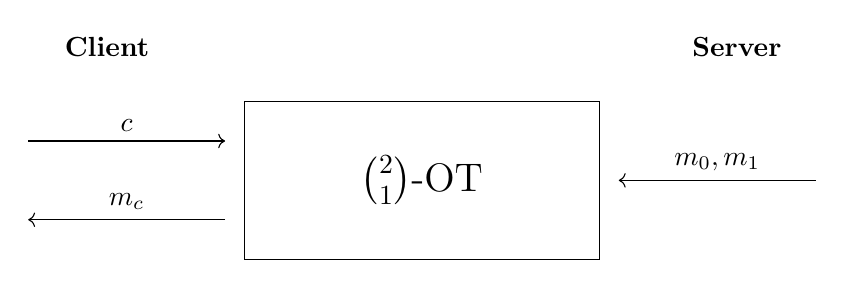
\begin{tikzpicture}
     \node[text centered] at (-4, 1.7) {\textbf{Client}};
     \node[text centered] at (4, 1.7) {\textbf{Server}};

     \node[draw, text centered, minimum width= 4.5cm, minimum height=2cm] at
       (0,0){\Large{$2\choose 1$-OT}};
     \draw[->](5, 0) -- (2.5, 0)node[midway,above]{$m_0, m_1$};

     \draw[->] (-5, 0.5)  -- (-2.5, 0.5) node[midway,above]{$c$};
     \draw[->] (-2.5, -0.5) -- (-5, -0.5) node[midway,above]{$m_{c}$};
   \end{tikzpicture}
   \pause

   \vspace{1em}
   \alert{Extend} with symmetric operations!
 \end{frame}

 \begin{frame}{A little help from MPC friends (cont.)}
   \centering
   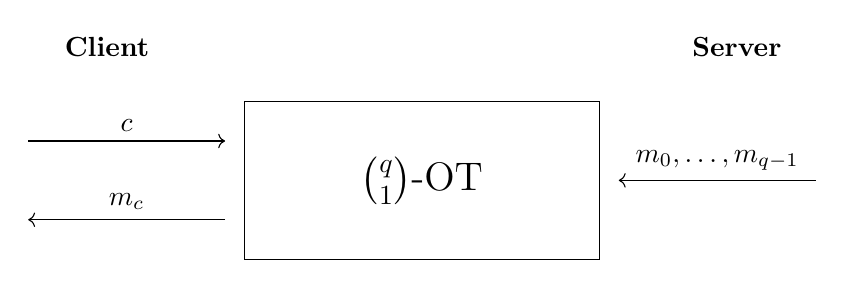
\begin{tikzpicture}
     \node[text centered] at (-4, 1.7) {\textbf{Client}};
     \node[text centered] at (4, 1.7) {\textbf{Server}};

     \node[draw, text centered, minimum width= 4.5cm, minimum height=2cm] at
       (0,0){\Large{$q\choose 1$-OT}};
     \draw[->](5, 0) -- (2.5, 0)node[midway,above]{$m_0, \ldots, m_{q-1}$};

     \draw[->] (-5, 0.5)  -- (-2.5, 0.5) node[midway,above]{$c$};
     \draw[->] (-2.5, -0.5) -- (-5, -0.5) node[midway,above]{$m_{c}$};
   \end{tikzpicture}
   \pause

   \vspace{1em}
   Generic construction from \alert{${\log q}$ $2\choose 1$-OTs} !
 \end{frame}

 \begin{frame}{A little help from MPC friends (cont.)}
   \centering
   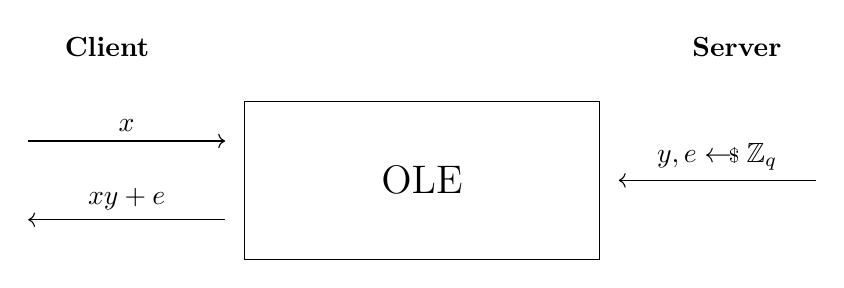
\begin{tikzpicture}
     \node[text centered] at (-4, 1.7) {\textbf{Client}};
     \node[text centered] at (4, 1.7) {\textbf{Server}};
     \node[draw, text centered, minimum width= 4.5cm, minimum height=2cm] at
       (0,0){\Large{OLE}};
     \draw[->](5, 0) -- (2.5, 0)node[midway,above]{$y, e\sample \ZZ_q$};

     \draw[->] (-5, 0.5)  -- (-2.5, 0.5) node[midway,above]{$x$};
     \draw[->] (-2.5, -0.5) -- (-5, -0.5) node[midway,above]{$xy+e$};
   \end{tikzpicture}
   \pause

   \vspace{1em}
   Generic construction from \alert{${\log q}$ $2\choose 1$-OTs} !
 \end{frame}
 %
 %   %%%%%%%%%%%%%%%%%%%%%%%%%%%%%%%%%%%%%%%%%%%%%%%%%%%%%%%%%%%%%%%%%%
 %
 \begin{frame}{Leap}
   \begin{itemize}
     \item Leap~\cite{EC:HKLMRR25}: Naor-Reingold LWR OPRF! \pause
     \item very fast online: can shift almost everything to the preprocessing phase\pause
     \item online phase takes less than a millisecond\pause
     \item \emph{symmetric-style} evaluation\pause
     \item optimized for PSI
   \end{itemize}
 \end{frame}

 \begin{frame}{An OPRF from \textsc{Spring}}
   \begin{columns}
     \hspace*{0.1em}
     \vspace*{-3em}
     \begin{column}{.48\textwidth}
       \begin{figure}
         \begin{align*}
           \only<1-2>{
             \color{colC}S\left(\intt\left(\mathsf{lookup}\left(\color{black}\kkk_0+
             \sum_{i=1}^m {c_i}\kkk_{i}\color{colC}\right)\right)\right)
           }
           \only<3-5>{
             \color{colC}S\left(\intt\left(\color{black}\mathsf{lookup}\left(\kkk_0+
             \sum_{i=1}^m {c_i}\kkk_{i}\right)\color{colC}\right)\right)
           }
           \only<6-7>{
             \color{colC}S\left(\color{black}\intt\left(\mathsf{lookup}\left(\kkk_0+
             \sum_{i=1}^m {c_i}\kkk_{i}\right)\right)\color{colC}\right)
           }
           \only<8->{\color{black}
             S\left(\intt\left(\mathsf{lookup}\left(\kkk_0+ \sum_{i=1}^m {c_i}\kkk_{i}\right)\right)\right)
           }
         \end{align*}
       \end{figure}
     \end{column}
     \begin{column}{.67\textwidth}
       \centering
       \vspace*{-3em}
       \resizebox{\textwidth}{!}{
         \begin{tikzpicture}[background rectangle/.style={fill=mBGcol}, show
           background rectangle]
           % Label for Client on the left and Server on the right
           \uncover<1->{
             \node[text centered] at (-4, 2) {\textbf{Client}};
             \node[text centered] at (-4, 1.4) {$\bv{c}=[c_1, \ldots, c_m] \in
               \{0,1\}^m$};
             \node[text centered] at (4, 2) {\textbf{Server}};
             \node[text centered] at (4, 1.4) {$\bv{K}=[\kkk_0, \kkk_1, \ldots, \kkk_m] \in
               \{0,1\}^m$};

             \node[draw, text centered, minimum width= 4.5cm, minimum height=2cm] at
               (0,0){\Large{$2\choose 1$-OT}};
             \draw[->](5, 0) -- (2.5, 0)node[midway,above]{$\bv{r}_i, \bv{r}_i+\kkk_i$};

             \draw[->] (-5, 0.5)  -- (-2.5, 0.5) node[midway,above]{$c_i$};
             \draw[->] (-2.5, -0.5) -- (-5, -0.5) node[midway,above]{$\bv{r}_i+\kkk_i{c_i}$};

           }
           \uncover<2->{
             \draw[line width=0.1 mm] (-5.5,-1.1) -- (5.5,-1.1);
             \node[ text centered, minimum width= 4.5cm, minimum height=1cm] at
               (0,-1.5){$\sum_{i=1}^\kappa \bv{r_i}+c_i \bv{k_i}$\qquad  \qquad\qquad\qquad
               $\kkk_0-(\sum_{i=1}^\kappa \bv{r}_i)$};
           }
           \uncover<3->{
             \node[ text centered, minimum width= 4.5cm, minimum height=1cm] at
               (0,-1.8){\faRecycle};
             \draw[line width=0.2 mm] (-5.5,-2.8) -- (5.5,-2.8);
             \node[ text centered, minimum width= 4.5cm, minimum height=1cm] at
               (0,-2.3){$\bv{b}\leftarrow\prod_{i=1}^\kappa \bv{r_i}\bv{k_i}^{c_i}$\qquad  \qquad\qquad\qquad
               $\bv{a}\leftarrow\kkk_0(\prod_{i=1}^\kappa \bv{r}_i)^{-1}$};
           }
           \uncover<4->{

             \node[draw, text centered, minimum width= 4.5cm, minimum height=2cm] at
               (0,-4){\Large{OLE}};
             \draw[->](-5, -3.6) -- (-2.5, -3.6) node[midway,above]{$b_i$};
             \draw[<-](-5, -4.5) -- (-2.5, -4.5)node[midway,above]{$y_i=a_ib_i+e_i$};
             \draw[<-] (2.5, -4)  -- (5, -4) node[midway,above]{$a_i,
                 e_i \sample
               \ZZ_q$};

             \draw[line width=0.1 mm] (-5.5,-5.1) -- (5.5,-5.1);
           }
           \uncover<5->{
             \node[ text centered, minimum width= 4.5cm, minimum height=1cm] at
               (-0.5,-5.5){$\bv{y}\leftarrow\sum_{i=0}^{n-1} (a_i\cdot b_i + e_i) X^i$\qquad \qquad  \qquad\quad
               $\bv{e}\leftarrow\sum_{i=0}^{n-1} e_i X^i$};
           }
           \uncover<6->{
             \node[ text centered, minimum width= 4.5cm, minimum height=1cm] at
               (0,-6){$\intt$};
           }
           \uncover<7->{
             \node[ text centered, minimum width= 4.5cm, minimum height=1cm,
               visible on=<9->] at
               (0.1,-6.5){\qquad\qquad\qquad\qquad\qquad\qquad\qquad\qquad
               $\bv{d}\sample\{0,1\}^n$};
             \draw[line width=0.2 mm] (-5.5,-7) -- (5.5,-7);
           }
           \uncover<8->{
             \node[draw, text centered, minimum width= 4.5cm, minimum height=2cm] at
               (0,-8.5){\Large{$q\choose 1$-OT}};

             \draw[->](-5, -8) -- (-2.5, -8) node[midway,above]{$y_i$};
             \draw[<-, visible on=<8>](-5, -9) -- (-2.5, -9) node[midway,above]{$\lfloor
               y_i-e_i\rceil_p$};
             \draw[<-, visible on=<9->](-5, -9) -- (-2.5, -9) node[midway,above]{$\lfloor
               y_i-e_i\rceil_p\oplus d_i$};
             \draw[->, visible on=<8>](5, -8.5) -- (2.5, -8.5) node[midway,above]{$\lfloor
               (q_i-e_i)\rceil_p $} ;
             \draw[->, visible on=<9->](5, -8.5) -- (2.5, -8.5) node[midway,above]{$\lfloor
                 (q_i-e_i)\rceil_p\oplus d_i
               $} ;
             \node [text centered] at (4, -9){$ \forall q_i\in \ZZ_q$};
           }
           \uncover<9->{
             \draw[<-, visible on=<9->](-4, -10.25) -- (4, -10.25)
               node[midway,above]{$\mathsf{BCH(\bv{d})}$};
           }
         \end{tikzpicture}

       }
     \end{column}
   \end{columns}
 \end{frame}

  \begin{frame}{Conclusion}
    \begin{itemize}
      \item Leap has a proof in the semi-honest model\pause \\
        Some problems to make it malicious secure. \pause
      \item Parameter choice may be sub-optimal.\pause
      \item Planning to do cryptanalysis on symmetric variant mod 16 \pause
      \item Quesions? Ideas? Let's discuss! \\

    \end{itemize}
  \end{frame}
 

 %   \begin{frame}{I am very proud of it}
 %     \begin{itemize}
 %       \item[\faCheck] proof in the semi-honest model\pause
 %       \item two problems make it hard to claim
 %         malicious security
 %     \end{itemize}
 %   \end{frame}
 % 
 %   \begin{frame}{Server Attack}
 %     \begin{itemize}
 %       \item generic attack on Naor-Reingold OPRFs \pause
 %       \item only works when the server can
 %         reason about the OPRF output \pause
 %       \item either because it is revealed later or because the
 %         protocol gives information (e.g. whether or not an authentication attempt
 %         succeeds.)  \pause
 %     \end{itemize}
 % 
 %     \begin{example}[Generic Attack on Naor-Reingold OPRFs]
 %       Instead of honestly inputting $\kkk_i+\bv{r}_i$ into the $2\choose 1$-OT, a
 %       malicious server may input some $\Delta_i+\bv{r_i}$ for some $\Delta_i \neq
 %       \kkk_i$. When the client result is revealed, the server can learn whether or not the
 %       $i^{th}$ bit is set.
 %       %  For example, if the authentication
 %       %  succeeds even though the server inputted $\bv{\Delta}_i$, the server can
 %       %  conclude that the $i^{th}$ bit of the client is not set. If the authentication
 %       %  attempt fails, the bit may be set. This is less reliable as the client may have
 %       %  just mistyped the password, but over multiple runs (e.g. by faulting the other
 %       %  message) the server can be more sure.
 %     \end{example}\pause
 %     Solution? \emph{verifiable}
 %     variant of this OPRF. But:
 %     Naor-Reingold keys are rather large which makes the verification less efficient.
 %   \end{frame}
 % 
 %   \begin{frame}{Client Attack}
 %     \begin{itemize}
 %       \item leak public key coefficients by faulting the rounding step of
 %         the OPRF\pause
 %       \item The key observation is that the rounding result is \emph{deterministic
 %         and constant for fixed inputs}\pause
 %       \item add an offset $\Delta$ to the coefficient and leak the exact point where the rounding
 %         result flips from zero to one or vice versa. \pause
 %       \item
 %         The attack is mitigated by enforcing \emph{consistency} between the OLE output
 %         and the rounding input so the client cannot compute the offset anymore.
 %     \end{itemize}
 %   \end{frame}
 % 


 \begin{frame}[allowframebreaks]
   \frametitle{References}

   \bibliography{bilbio,cryptobib/crypto,cryptobib/abbrev3}
   \bibliographystyle{alpha}

 \end{frame}
 %  \section{Post-Quantum OPRFs}
 %  % Current state: Elliptic curve OPRFs (e.g., OPAQUE, VOPRF standard)
 %  % The quantum threat: Why we need PQ alternatives
 %  % The efficiency problem: Why existing PQ constructions struggle
 %  % 
 %  % Lattice-based attempts require heavy ZK proofs
 %  % Often no better than using blind signatures
 %  % Set up the question: Can we do better?
 % 

 % Lattice-based cryptography essentials (brief, assume some familiarity)
 % Oblivious Transfer: the key enabling primitive
 % 
 % Why OT is "cheaper" than ZK proofs in the PQ setting


 % The core insight: Eliminate ZK proofs entirely
 % High-level construction overview
 % 
 % Oblivious evaluation of lattice-based PRF via OT
 % The preprocessing phase (acknowledge the overhead upfront)
 % The online evaluation phase
 % 
 % 
 % Performance characteristics: where Leap wins and where it pays costs
 % The sweet spot: repeated executions (PSI and similar applications)

 % \section{A story of failure: Two and a half attacks}
 % "Now let's look under the hood at what makes this work..."
 % Segue: The PRF at the heart of Leap can be expressed as a binary circuit, which connects nicely to symmetric cryptanalysis perspectives...
 % 
 % This should take about 20-25 minutes depending on your pacing, leaving you well-positioned to dive into the circuit representation and connect to their symmetric crypto interests in the second half.

 % 
 % \begin{frame}{Blind-evaluate-unblind paradigm}
 %   \begin{enumerate}
 %     \item The client hashes the input to the group, samples an invertible blinding
 %       element, and blinds the hashed element that is then sent to the server.\pause
 %     \item The server then faithfully evaluates the element with the key and
 %       returns the result.\pause
 %     \item The client unblinds the server result and has a PRF evaluation without
 %       having to reveal the input.\pause
 %   \end{enumerate}
 % 
 %   \hfill \alert{Task:} think about what could go wrong at each step
 % \end{frame}
 % 
 % \begin{frame}{Pre-quantum Blind-evaluate-unblind: 2HashDH}
 %   \vspace{-2em}
 %   \procedureblock[mode=text]{}{%
 %     \> \textbf{Client} \> \> \textbf{Server} \((k)\)\\
 %     \textbf{1. Init:}  \>              \> \sendmessageleft*[16em]{A \coloneqq k \cdot G}   \>\\
 %     \textbf{2. Query:} \> Sample \(r\) \> \sendmessageright*[16em]{B \coloneqq H(x) + r\cdot G} \> \\
 %     \> \(C-{r}\cdot{A}\) \> \sendmessageleft*[16em]{{C \coloneqq k \cdot B}}\\
 %     \> \(= {k}\cdot{H(x)} + {rk}\cdot{G} - {rk}\cdot{G}\)\\
 %     \> \(= {k}\cdot{H(x)}\)
 %     }
 % 
 %     %\alert{Hint:} This will not get easier with lattices.
 % \end{frame}
 % 
 % \begin{frame}{How would an ideal OPRF look like?}
 %   %gold standard: 3HashDH OPRF~\cite{EC:TCRSTW22}
 %   \begin{description}
 %     \item[Security.] ideally malicious security, i.e. a malicious adversary cannot
 %       learn anything they shouldn't \pause (doesn't imply detection)\pause
 %     \item[Round-Optimality.] A \alert{round} is a period where all parties can
 %       exchange messages simultaneously. \\ \pause A non-interactive protocol (e.g.  NIZK):
 %       single round, interactive protocol: two rounds \pause
 %     \item[Communication size.] Elliptic curve OPRFs: 766
 %       bits of communication. Best lattice-based: tens of kilobytes, in
 %       a semi-honest setting and with preprocessing.\pause
 %     \item[Computational complexity.] Generic lattices are fast, and we can speed them up
 %       further using vector instructions or even GPUs. \\\pause
 %       Kyber768 takes between a third to half of the
 %       computational time of ECDH Curve 25519!
 %   \end{description}
 % \end{frame}
 % \begin{frame}{Anything else?}
 %   \begin{description}
 %     \item[Preprocessing.]  Repeated
 %       computations? Shift data-independent communication and computation to a
 %       preprocessing phase.  \pause Fully online protocols: online variant or
 %       perform the precomputation on the fly.\pause
 %     \item[Trusted Setup.] In addition to preprocessing, some OPRFs rely on a
 %       trusted setup.\pause But: trust is a hard problem in itself,
 %       and sometimes a trusted setup just isn't available (e.g. for
 %       CSIDH).
 %   \end{description}
 % \end{frame}
 % 
 % \sectionheader{OPAQUE and Private Set Intersection} % dark background
 % 
 % \begin{frame}{OPAQUE}
 %   \vspace{-3em}
 %   \procedureblock[mode=text]{}{%
 %     \> \textbf{Client} (pwd)  \> \> \textbf{Server} (k)\\
 %     \textbf{1. Registration:} \> \(k' = F_{k}(pwd)\) \> \sendmessagerightleft*[16em]{OPRF} \> \\
 %     \> Sample \((pk, sk)\) \> \sendmessageright*[16em]{pk, ct=Enc_{k'}(sk)} \> Store \((pk, ct)\)\\
 %     \uncover<2->{
 %       \textbf{2. Login:} \>\>\sendmessageleft*[16em]{ct} \>\\
 %       \> \(k' = F_{k}(pwd)\) \>\sendmessagerightleft*[16em]{OPRF} \> \\
 %       \> \(sk = Dec_{k'}(ct)\) \>\sendmessagerightleft*[16em]{\text{AKE using }sk} \>
 %     }
 %     }
 %     \uncover<3->{
 %       \hspace*{\fill} \alert{Task: Which properties are important?}
 %     }
 % \end{frame}
 % 
 % \begin{frame}{OPAQUE: Properties}
 %   \begin{itemize}
 %     \item doesn't reveal output\pause
 %     \item server still passively observes the success or failure of an authentication
 %       attempt\pause
 %     \item OPRF must be secure against a malicious server\pause
 %     \item Verifiability?
 %   \end{itemize}
 % \end{frame}
 % 
 % 
 % \begin{frame}{Private Set Intersection~(PSI)}
 %   OPRFs are useful for \alert{unbalanced} sets, where one party, typically the
 %   server in client-server protocols, has a significantly larger set than the other party.
 %   \begin{figure}
 %     \centering
 %     \procedureblock[mode=text]{}{%
 %       \textbf{Alice} \((x_{1}, \ldots, x_{m})\) \> \> \textbf{Bob} \((y_1,
 %       \ldots, y_n), k\)\\
 %       \({\{F_{k}(x_i)\}}_{i \in [m]}\) \> \sendmessagerightleft*[16em]{OPRF
 %       } \> \\
 %       \> \sendmessageleft*[16em]{\{z_j = F_k(y_i)\}_{j \in [n]}} \>\\
 %       }
 %       \(F_{k}(x_i) = z_{j}\).
 %       Otherwise \(F_{k}(y_j)\) is pseudorandom.
 %   \end{figure}\pause
 %   \hspace*{\fill} \alert{Task: Which properties are important?}
 % \end{frame}
 % 
 % \begin{frame}{PSI: Properties}
 %   \begin{itemize}
 %     \item per-client keys may cause segmentation \pause
 %     \item semi-honest server may be realistic: \pause
 %       \begin{itemize}
 %         \item regulatory and reputational incentives~\cite{USENIX:KRSSW19}\pause
 %         \item inherent trust\\ government agencies identifying duplicate entries\pause
 %         \item anywhere where PSI is applied to limit the risk of data breaches
 %       \end{itemize}
 %   \end{itemize}
 % \end{frame}
 % 
 % \sectionheader{2HashDH from lattices} % dark background
 % \begin{frame}{How to get a 2HashDH lattice OPRF? }
 %   \begin{table}[!ht]
 %     \centering
 %     \fbox{
 %       \begin{tabular}{ll}
 %         \toprule
 %         Discrete Logarithm &  Ring-LWE \\
 %         \midrule
 %         $g$ & $\bv{a}$\\
 %         $g^x$ & $\bv{a} \bv{s} + \bv{e}$\\
 %         $g^x g^y = g^{x+y}$ &  $(\bv{a} \bv{s} + \bv{e}_0) + (\bv{at} + \bv{e1}) =
 %         \bv{a}(\bv{s} + \bv{t}) + \bv{e'}$\\
 %         $(g^a)^b = (g^b)^a$ & $(\bv{as} + \bv{e}) \bv{t} = (\bv{a s t} + \bv{et})\approx \bv{a s t} \approx (\bv{a t} + \bv{e})\bv{s}$\\
 %         $(g, g^a, g^b, g^{ab})$ &  $(\bv{a}, \bv{as} + \bv{e}, \bv{at} + \bv{d},
 %         \bv{ast} + \bv{e'})$\\
 %         $\approx_c (g, g^a, g^b, u)$ & $\approx_c (\bv{a}, \bv{as} + \bv{e},
 %         \bv{a t} + \bv{d}, \bv{u})$\\
 %         \bottomrule
 %       \end{tabular}
 %     }
 %     \caption{Martin Albrechts \textit{DH to Ring-LWE Dictionary}
 %     \url{https://martinralbrecht.wordpress.com/2021/05/07/round-optimal-verifiable-oblivious-pseudorandom-functions-from-ideal-lattices/\#more-1910}.
 %     $\bv{s},\bv{t},\bv{e}_0,\bv{e}_1,\bv{e'},\bv{d},\bv{e}$ are small elements in
 %     the lattice.
 %     }
 %     \label{tab:dict}
 %   \end{table}
 % \end{frame}
 % 
 % 
 % \begin{frame}{Lattice-based 2HashDH OPRF}
 %   \vspace{-1em}
 %   \begin{figure}[!ht]
 %     \procedureblock[mode=text]{}{%
 %       \> \textbf{Client} \> \> \textbf{Server} \((k)\)\\
 %       \textbf{1. Init:}  \>              \> \sendmessageleft*[22em]{c \coloneqq a \cdot \underline{k} + \underline{e_0},\  a \in \ZZ_{q}[X]/(X^N + 1)} \>\\
 %       \textbf{2. Query:} \> Sample short \(\underline{r}\) \> \sendmessageright*[22em]{c_{x} \coloneqq H(x) + a \cdot \underline{r} + \underline{e_1}} \> \\
 %       \> \(y \coloneqq d_x-c\cdot\underline{r}\) \> \sendmessageleft*[22em]{{d_{x} \coloneqq c_{x} \cdot \underline{k} + \underline{e_2} = (H(x) + a \cdot \underline{r} + \underline{e_1})\cdot\underline{k} + \underline{e_2}}}
 %       }
 %       \[d_x-c\cdot\underline{r}= H(x)\cdot\underline{k} + a\cdot{rk} + \underline{e_1\cdot{k}} + \underline{e_2} - a\cdot{rk} - \underline{e_{0} \cdot r} \approx H(x) \cdot {k}\]
 % 
 %       \caption{Generic construction for 2HashDH OPRF from LWE~\cite{PKC:ADDS21}.
 %       \underline{Underlined} variables are short. }
 %   \end{figure}
 %   \hfill\alert{Task} What do we have to prove?
 % \end{frame}
 % 
 % \begin{frame}{How could a malicious client attack when we forego ZK? }
 %   \begin{itemize}
 %     \item Is it safe to output $c_x\bv{k}+\underline{\bv{e}}$ for arbitrary
 %       $c_x$?\pause ~no, trapdoors!\pause
 %     \item Noise Leakage: the client learns $\bv{e}_1\bv{k}+\bv{e}_2-\bv{e}_0\bv{ r}$
 %       where they choose $\bv{e}_0$ and $\bv{r}$ before rounding.
 %     \item \alert{Task} What could be recovered from the leakage?
 %   \end{itemize}
 % \end{frame}
 % 
 % \begin{frame}{How could a malicious client attack when we forego ZK? }
 %   As it turns out, there is a trivial
 %   attack:
 %   \begin{itemize}
 %     \item Write $\bv{a} \coloneqq (\bv{e}, \bv{-r})$ and $s \coloneqq (\bv{k}, \bv{e}_0)$
 %     \item Rewrite
 %       $\bv{e}_c \bv{k} + \bv{e}_0 - \bv{e}_s \bv{r}$
 %       as $\bv{as} + \bv{e_1}$\pause
 %     \item This is essentially an instance of \emph{LWE without modular
 %       reduction}!~\cite{AC:BDEFT18} which is easy. \footnote{
 %         This is a bit of a simplification because $\bv{e_1}$ is sampled fresh in each
 %         invocation so the attack does not apply directly.}
 %   \end{itemize}
 % \end{frame}
 % 
 % \begin{frame}{Client Proof}
 %   The OPRF requires the client to prove in zero-knowledge that the
 %   initial message
 %   $\bv{c}_x \coloneqq H(x) + \bv{ar} + \bv{e}_1$ is \emph{well-formed}.\pause
 % 
 %   More concretely, the client has to prove that:
 %   \begin{itemize}
 %     \item they know an $\bv{x}\in \{0,1\}^\kappa$ \pause
 %     \item $\bv{r}\in R$ is a small element with $\ll \bv{r} \ll_\infty \leq \sigma \sqrt{n}$\pause
 %     \item $\bv{e}_1\in R^{1\times \ell}$  where $\ll\bv{e}_1\ll_\infty \leq \sigma
 %       \sqrt{n}$\pause
 %   \end{itemize}
 %   \alert{Task} Which proof is most expensive? \pause
 %   The first one.
 % 
 % \end{frame}
 % 
 % \begin{frame}{Server proof}
 %   The server has two proofs:
 %   \begin{enumerate}
 %     \item in the initialization phase that proves
 %       knowledge of a key $\kkk\in R$ and an error term $\bv{e}_0\in R^{1\times
 %       \ell}$,\pause ~
 %       both of which are shorter elements, \pause and that the key commitment $\bv{c}\coloneqq
 %       \bv{a} k +\bv{e}_0$ contains $\bv{a}$
 %       such that the commitment is well-formed $\bv{c}=\bv{a}k+\bv{e}_0 \mod q$\pause
 %       \begin{itemize}
 %         \item can be removed by trapdooring $\kkk$!\pause
 %         \item  $\kkk$ has to be extractable, which is also possible by using a
 %           trapdoor. However, the proof isn't that bad. \pause
 %       \end{itemize}
 %     \item  prove that $\bv{d}_x=\bv{c}_xk+\bv{e}_2 \mod q$ \\
 %       Note that the proof can be amortized: batch several queries and use the
 %       same ZKP instance for all.
 % 
 %   \end{enumerate}
 % \end{frame}
 % 
 % 
 % \begin{frame}{Removing the $2^{nd}$ server proof: Verifiability with Cut-and-Choose}
 %   We can
 %   use a generic transformation with combinatorial arguments to detect a cheating
 %   server.\pause
 %   \begin{itemize}
 %     \item Request $a$ OPRF evaluations two rounds, some of them with your actual
 %       input $x$.\pause
 %     \item Select $y$ points, submit in clear and request prove that these are well-formed\pause
 %     \item Argue combinatorially about adversarial success\pause
 %   \end{itemize}
 %   Main Problem: converts a round-optimal OPRF to a four-round VOPRF.
 % \end{frame}
 % 
 % \begin{frame}{Bottlenecks}
 %   \begin{enumerate}
 %     \item correctness requirements on the ring modulus
 %       \begin{itemize}
 %         \item semihonest: 256-bit modulus and a ring dimension of $2^{14}$, which sums to about 2MB
 %           of communication (over 0.5 MB per ring element). \pause
 %         \item malicious secure correctness: 2048 bit modulus \pause
 %           prevent adversaries from maliciously sampling $k$ such that
 %           $H(x)k$ produces a rounding error. 1D-SIS assumption requires $q \gg
 %           2^{2\lambda}$. \pause
 %       \end{itemize}
 %     \item Statistical Noise Drowning
 % 
 %       \begin{itemize}
 %         \item \alert{Task} What is the size of the error terms $\bv{e}_1, \bv{e}_2$ ? \pause
 %         \item have to be small in relation to $q$: \\
 %           $
 %           q \overset{\text{correctness of }\approx}{\gg} \bv{e}_{s}
 %           \overset{\text{hide } \bv{k}}{\gg} \bv{e}_{c} \cdot \bv{k}
 %           $\pause
 %       \end{itemize}
 %     \item NIZKAoKs
 %       \begin{itemize}
 %         \item Efficiency gain from LaBRADOR~\cite{C:BeuSei23}
 %       \end{itemize}
 % 
 %   \end{enumerate}
 % \end{frame}
 %% 

 \end{document}
